\section{Introduction}
Robots moving in real-world scenarios need to be adaptable and reactive.
While on the one hand, the robot needs to complete its motion, on the other hand, its movement must be safe, i.e., it can avoid collisions at all times.
Modern robotic applications require increased physical human-robot collaboration \cite{ajoudani2018progress}.

One of the big tasks of controlling a robot is planning a trajectory to reach a desired goal. Trajectories can often be very complex, and one has to find methods to parametrize those easily. The human demonstration is an easy way of showing the robot what to do. Simple movement can be sequenced to generate a complex motion \cite{gribovskaya2011motion}.

It has a closed-form control law does not require constant replanning for every position. In addition, DS control can provide stability and convergence guarantees for navigation in dynamic environments.

Applications that involve interactions with an unknown and dynamic environment, for example, manipulation around humans, require controllers for actuators that are not which exceed classical stiffness controllers.

Biological muscles outperform mechanical devices in terms of functional and neuro-mechanical control. One key distinction is the adaptable compliance or variable stiffness exhibited in biological systems, which contrasts with the performance of traditional stiff electrical drives commonly used in industrial robotics. Unlike these drives, which rely on precise reference-trajectory tracking, biological systems possess inherent flexibility and adaptability.

Most reactive motion controllers do not specifically consider the task of obstacle avoidance. This is the advantage of impedance controllers; if designed correctly, the motion remains stable for collision avoidance. Additionally, the force applied to an external obstacle remains below a specified threshold. 
However, for improved behavior, the robot should avoid collisions proactively before they happen while the impedance control remains in the fail-safe interaction mode.

\begin{figure}
\centerline{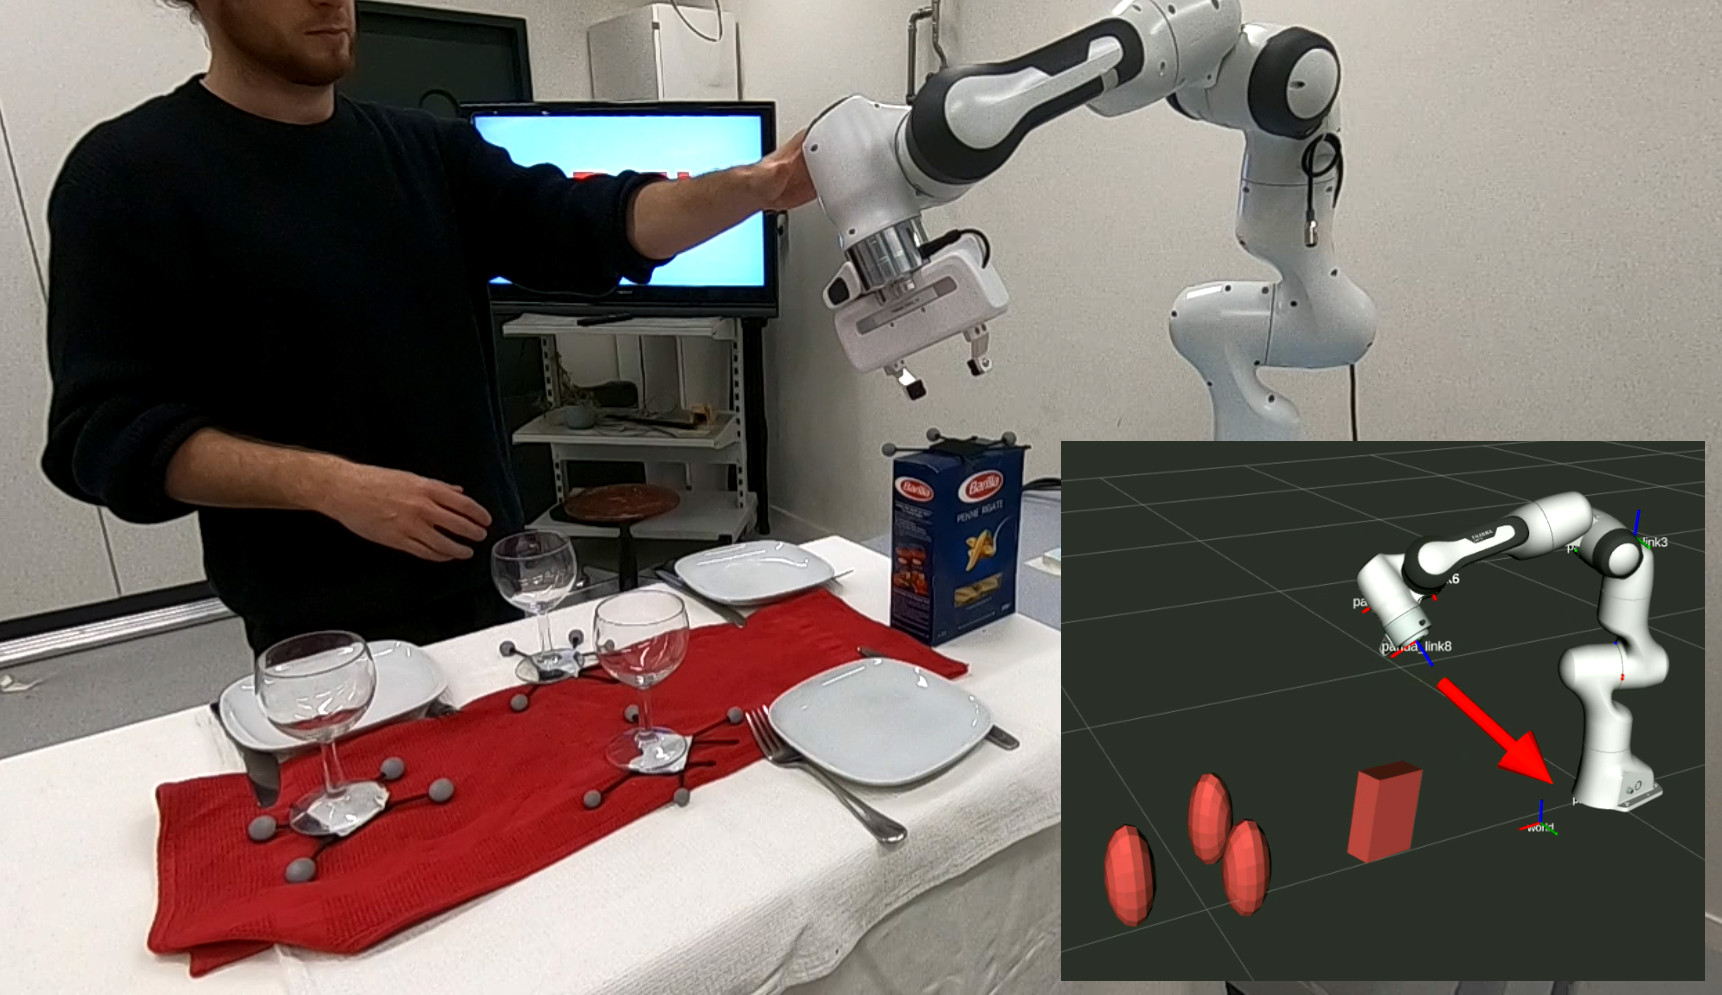
\includegraphics[width=0.5\textwidth]{figures/robot_arm_table_avoidance}}
\caption{Using the proposed obstacle aware passivity controller, the robot is able to safely avoid external disturbance and ensuring collision avoidance.}
\label{fig:table_avoidance_with_obstacle}
\end{figure}


\subsection{Literature Review}
\cite{takegaki1981new}
Impedance control is a feedback control algorithm that imposes a Cartesian impedance to the end-point of a nonlinear manipulator resulting \cite{hogan1985impedance}. This results in the elimination of the \textit{inverse kinematics problem} in favor of \textit{forward kinematics}.
Conversely, to position control algorithms, impedance control creates a dynamic relation between desired position, velocity, and force rather than controlling for these values individually.   
While the first impedance controller used constant stiffness, many approaches have been proposed for dynamic control parameters to have improved adaptation to the environment \cite{vanderborght2013variable, abu2020variable}. 
% older variable actuators focused review \cite{vanderborght2013variable}
% Progress and prospects of the human-robot collaboration \cite{ajoudani2018progress}

% Passive Controllers
Passive velocity field controllers first encode the desired task as a velocity field, approximating a damping control law, which tries to approximate the velocity \cite{li1999passive,}. However, the approach relies on a storage tank inspired by a virtual flywheel.

The approach is extended by providing more intuitive energy tanks to enable interaction with obstacles below the force limit \cite{kishi2003passive}.

The most recent approach uses impedance control based on selective dissipation of the energy \cite{kronander2015passive}. This method, called passive interaction control, allows the robot to be stiff or compliant depending on the direction of the disturbance.

Passivity analysis is often used for teleoperated systems to ensure safe operation during operation.
The first approach to the dynamics is slowly updating the desired position, coupled with a spring-damper model with an impedance controller for an interactive system
\cite{lee2010passive}.
A sampling-based approach has been used to provide passivity to a coupled system by analyzing the preserving passivity for the systems individually \cite{stramigioli2005sampled}.

Learning and continuously adapting the control parameters have been shown to improve the controller performance in direct human-robot collaboration
\cite{gribovskaya2011motion}.
However, the controller adaptation focuses on improving movement accuracy rather than rejecting disturbances.

A general framework can be used to ensure that position-, torque-, and impedance controllers exhibit passive \cite{albu2007unified}. By interpreting the torque feedback as the shaping of the motor inertia, the flexible robot arms can be used in complex interaction tasks, such as insertion or wiping.
Combining impedance controllers with admittance controllers allows for accurate yet cooperative control
\cite{fujiki2022series}.


% Energy tanks 
Impedance controllers are designed with time-varying stiffness to adapt the behavior from free motion to physical interaction with the environment  \cite{ferraguti2013tank}. However, such a system can become unstable, but virtual energy tanks can be used to ensure passivity.
Alternative approaches ensure the stability of variable impedance controllers by setting constraints on the damping and stiffness, as well as their rate of change \cite{kronander2016stability}.
% The controller was extended to have variable stiffness to favor task completion \cite{kronander2015passive}. However, both approaches rely on energy tanks for general, desired dynamics and do not give any guarantees in the presence of obstacles.


% Geometric Methods
Tracking controllers often require linearization or other simplification methods. However, \cite{udwadia2003new} develops a class of tracking controllers for exact control of the nonlinear mechanical systems at a low computational cost by reformulating control problems as a particular class of optimal controllers. With this method, several standard control problems in robotics can be derived \cite{peters2008unifying}.

The consistent combination of local Riemannian Motion Policies (RMP) is combined for globally stable force-controlled motion \cite{cheng2020rmp}.
New position-dependent Riemannian metrics improve the task design using RMP, allowing for reactive force control under constraints \cite{bylard2021composable}.

Geometric fabrics have been introduced as a mathematical tool for shaping the robot's nominal behavior, capturing constraints such as obstacle avoidance, joint limits, redundancy resolution
\cite{xie2020geometric}.
Finsler geometry combined with geometric fabrics has enabled increased path consistency \cite{ratliff2021generalized}.
Geometric fabric generalizes classical mechanical systems to form new physical behavior, which has been used for multi-obstacle avoidance on a 7DoF robot arm \cite{van2022geometric}.
However, the geometric methods remain challenging to parameterize and can create unwanted motion artifacts.
 
% Real-time perception meets reactive motion generation \cite{kappler2018real} -> no real feedback on the collision avoidance level ?!

% AFP / Obstacle avoidance / Motion Control
In dynamic environments, obstacle avoidance is crucial for safe navigation. Early approaches used repulsive force fields from robots to avoid collisions of robotic manipulators \cite{khatib1987unified}. 
As this approach is prone to local minima, the elastic band's method has been introduced. Interpreting the initial trajectory as an elastic band and stretching the path around obstacles improves convergence  
\cite{
brock2002task, % Corresponding conference paper
brock2002elastic}.
Passive controllers have been designed to track the curve of the general potential field. The controller compensates for Coriolis and centrifugal forces. However, the method does not provide insurance of disturbance repulsion around obstacles \cite{duindam2004passive}. 
The additional usage of circular fields \cite{singh1996real} allows force-controlled navigation in cluttered environments with increased convergence for simple obstacles
\cite{haddadin2011dynamic}.
This has been combined with force-controlled navigation for manipulators \cite{tulbure2020closing}. However, the method was limited to convex meshes and cannot guarantee the absence of local minima in space.

% Dynamical system based avoidance + control
Alternatively, in our previous work \cite{huber2019avoidance, huber2023avoidance}, we introduced collision avoidance inspired by a harmonic potential. We ensured the absence of local minima in free space and enabled navigation around complex scenarios with star-shaped obstacles.
For implementation on the real robot, a passive controller stays close to the initial dynamics \cite{kronander2015passive}. However, the passive controller does not take into account its physical surrounding, and disturbances in the proximity of obstacles could lead to collisions.

Although DS passive-controlled robots work well in some simple cases, they do not yet have a reliable way of safely navigating through an obstacle environment. This issue could lead to collisions if unknown disturbances push the agent toward an obstacle. This work presents a method to address this problem by modifying the passive control law design. The resulting controller is now aware of its environment.

\subsection{Contribution}
In this work, we introduce the following contributions:
\begin{itemize}
\item A passive controller which ensures obstacle avoidance (Section~\ref{sec:obstacle_aware_passivity})
\item A passivity analysis without the need for storage tank which holds for a general damping controller for stable vector fields (Theorem~\ref{theorem:passivity})
\item A collision avoidance analysis which provides insight into the path consistency around obstacles (Section~\ref{sec:collision_avoidance})
\item Implementation and test on real robots (Section~\ref{sec:evaluation})
\end{itemize}
